% Comprehensive, accessible report for SIMC 2026 Question 3 (parts a-h).
% Compile with XeLaTeX (uses the system Times New Roman font), TWO passes for the
% table of contents and cross-references.  Run from the repository root:
%   xelatex -output-directory=doc doc/Q3_full_report.tex   (x2)
\documentclass[11pt]{article}

\usepackage[a4paper,margin=2.3cm]{geometry}
\usepackage{amsmath,amssymb,amsthm}
\usepackage{fontspec}
\setmainfont{Times New Roman}
\usepackage{graphicx}
\usepackage{booktabs}
\usepackage{xcolor}
\usepackage[hidelinks]{hyperref}
\usepackage[font=small,labelfont=bf]{caption}
\usepackage{enumitem}
\setlist{nosep,leftmargin=1.4em}

\graphicspath{{doc/FINAL/figs/}{FINAL/figs/}{figs/}}
\setlength{\parskip}{3pt}
\renewcommand{\arraystretch}{1.15}

\DeclareMathOperator{\tr}{tr}
\DeclareMathOperator{\Var}{Var}
\DeclareMathOperator{\Cov}{Cov}
\newcommand{\R}{\mathbb{R}}
\newcommand{\Xt}{\widetilde{X}}
\newcommand{\xt}{\widetilde{x}}
\newcommand{\Nt}{\widetilde{N}}
\newcommand{\norm}[1]{\lVert #1 \rVert}
\newcommand{\T}{^{\mathsf{T}}}

\theoremstyle{definition}\newtheorem{definition}{Definition}[section]
\theoremstyle{plain}\newtheorem{proposition}{Proposition}[section]
\theoremstyle{remark}\newtheorem{remark}{Remark}[section]

\title{\bfseries Question 3 --- A Complete Report\\[4pt]
\large Cleaning, Principal Component Analysis, and Clustering\\ of a High-Dimensional Spectroscopic Dataset}
\author{SIMC 2026 Endeavour Challenge \quad (Parts a--h)}
\date{May 2026}

\begin{document}
\maketitle

\begin{abstract}\noindent
This report works through the whole of Question 3 in detail and from the ground up. We are
given a table of $1000$ infrared spectra, each recorded at $3401$ frequencies, and asked to
clean it, analyse it, and ultimately recover how many distinct food samples it contains. Along
the way we meet --- and carefully define --- the row norm, mean-centering, variance, the
covariance and Gram matrices, eigenvalues and eigenvectors, Principal Component Analysis (PCA),
the singular value decomposition, cosine similarity, and clustering. The headline results are:
$40$ blank vials and $36$ anomalous high-norm vials are removed (leaving $924$ clean spectra);
the data is strongly low-dimensional, with a dominance ratio $\lambda_1/\lambda_2\approx3.53$
and a clear ``elbow'' at $k^\star=8$ signal directions; the leading principal direction is an
interpretable contrast between molecular bands; and clustering --- carried out two independent
ways that we prove must agree --- shows the genuine vials fall into well-separated groups of
about $37$ repeats each, giving a final count of \textbf{26 unique food samples}.
\end{abstract}

\tableofcontents
\bigskip

% ======================================================================
\section{Introduction and roadmap}\label{sec:intro}

Imagine a blind taste test. A thousand small vials are filled with fermented, caffeinated
drinks --- kombucha, cocoa drinks, coffee liqueurs, Chinese tea --- and an instrument shines
infrared light of many different frequencies through each one, recording how strongly the
liquid absorbs at each frequency. The result is a long list of numbers per vial, a
\emph{spectrum}, which acts as a chemical fingerprint. The labels saying which vial held which
drink have been lost, and our job is to use linear algebra to reconstruct the structure of the
experiment: which measurements are corrupt, which frequencies carry information, what the
dominant patterns of variation are, and --- finally --- how many genuinely different drinks
were tested.

The mathematics needed is introduced as we go, so no prior linear algebra is assumed. The
report is organised as follows. Section~\ref{sec:background} defines every tool we will use.
Section~\ref{sec:data} describes the dataset and a subtlety about how it is stored. Then each
part of Question 3 has its own section: cleaning (\S\ref{sec:3a}), variance and the covariance
matrix (\S\ref{sec:3b}), the eigenspectrum and PCA (\S\ref{sec:3c}), the leading eigenvector
(\S\ref{sec:3d}), clustering in two different spaces (\S\ref{sec:3e}--\ref{sec:3f}), the
comparison of those two approaches (\S\ref{sec:3g}), and the final count of unique samples
(\S\ref{sec:3h}). Section~\ref{sec:conclusion} ties the threads together, and the appendices
give a glossary and a table of all key numbers.

% ======================================================================
\section{Mathematical background, from scratch}\label{sec:background}

\subsection{Vectors and the norm}
A \textbf{vector} is just an ordered list of numbers, written as a column,
$x=(x_1,x_2,\dots,x_M)$. Each number is a \emph{component}. For us a single spectrum is a
vector of $M=3401$ absorbance values. The \textbf{(Euclidean) norm} of a vector measures its
overall size,
\[
  \norm{x} \;=\; \sqrt{x_1^2 + x_2^2 + \dots + x_M^2}.
\]
Geometrically it is the length of the arrow from the origin to the point $x$. Because every
component is squared before being summed, a few large values dominate the norm --- a fact we
exploit in Section~\ref{sec:3a}.

\subsection{Matrices, transpose, and products}
A \textbf{matrix} is a rectangular grid of numbers. The \textbf{transpose} $A\T$ is obtained by
swapping rows and columns, so $(A\T)_{ij}=A_{ji}$; a $p\times q$ matrix becomes $q\times p$.
The \textbf{dot product} of two vectors, $a\cdot b=\sum_i a_ib_i$, multiplies matching
components and adds them; it is large and positive when the two vectors point the same way,
zero when they are perpendicular. Matrix multiplication generalises this: entry $(i,k)$ of
$AB$ is the dot product of row $i$ of $A$ with column $k$ of $B$.

\subsection{The design matrix}
Our data is a \textbf{design matrix} $X\in\R^{N\times M}$ whose rows are \textbf{samples}
(one vial each) and whose columns are \textbf{features} (one frequency each); the entry
$X_{ij}$ is the absorbance of sample $i$ at frequency $j$. Here $N=1000$ and $M=3401$.

\subsection{Mean, variance, and mean-centering}
The \textbf{mean} of a feature is its average over the samples,
$\bar X_j=\tfrac1N\sum_i X_{ij}$. \textbf{Mean-centering} subtracts this average from every
entry of the column, producing $\Xt_{ij}=X_{ij}-\bar X_j$; afterwards every feature averages
zero. The \textbf{variance} of a feature is the average squared distance from its mean,
$\Var_j=\tfrac1N\sum_i(X_{ij}-\bar X_j)^2$. A large variance means the feature swings widely
between vials and is therefore informative; a near-zero variance means it is almost constant
and tells us little.

\subsection{The covariance matrix}
The \textbf{covariance} of two features asks whether they move together. Collected for all
pairs of the (mean-centred) features, the covariances form the \textbf{covariance matrix}
\[
  C \;=\; \tfrac1{\Nt}\,\Xt\T\Xt \;\in\;\R^{M\times M}, \qquad
  C_{ij}=\tfrac1{\Nt}\sum_{k}\Xt_{ki}\Xt_{kj}.
\]
An off-diagonal entry is positive when two features rise and fall together, negative when one
rises as the other falls. The diagonal entry $C_{jj}$ is the covariance of a feature with
itself, which is exactly its variance. Crucially, $C$ is \emph{symmetric}: $C\T=C$.

\subsection{Eigenvalues and eigenvectors}
For a square matrix $C$, a non-zero vector $v$ is an \textbf{eigenvector} with
\textbf{eigenvalue} $\lambda$ if
\[
  Cv=\lambda v,
\]
meaning that multiplying by $C$ only \emph{stretches} $v$ (by the factor $\lambda$) without
rotating it. Eigenvectors are the special, ``natural'' directions of a matrix.

\subsection{The spectral theorem and positive semi-definiteness}
Two facts about our $C$ make everything well behaved. By the \textbf{spectral theorem}, a real
symmetric matrix has only \emph{real} eigenvalues and a complete set of mutually perpendicular
(\textbf{orthonormal}) eigenvectors --- a clean coordinate system. And $C$ is \textbf{positive
semi-definite (PSD)}: for every vector $w$, $w\T C w\ge0$ (because, as we show later, it equals
a sum of squares). A PSD matrix has all eigenvalues $\ge0$, so each eigenvalue is a genuine,
non-negative variance.

\subsection{Principal Component Analysis (PCA) in one paragraph}
\textbf{PCA} is simply the eigendecomposition of the covariance matrix. Its eigenvectors are
the \emph{principal directions} of the data --- the axes along which the samples vary most ---
and the corresponding eigenvalues say how much variance lies along each. Keeping only the few
largest directions compresses the data while preserving almost all of its structure.

\subsection{The singular value decomposition and the Gram matrix}
Every matrix factors as $\Xt=U\Sigma V\T$ (its \textbf{singular value decomposition}, SVD),
where $U$ and $V$ have orthonormal columns and $\Sigma$ is diagonal with the non-negative
\emph{singular values} $\sigma_i$. The columns of $V$ are the eigenvectors of
$\Xt\T\Xt$ (feature space) and the columns of $U$ are the eigenvectors of the
\textbf{Gram matrix} $G=\tfrac1{\Nt}\Xt\Xt\T\in\R^{\Nt\times\Nt}$ (sample space); both have
eigenvalues $\sigma_i^2/\Nt$. The Gram entry $G_{ij}$ is the similarity (dot product) between
samples $i$ and $j$. This shared-eigenvalue link (Question 2d) is the reason the two clustering
routes in \S\ref{sec:3e}--\ref{sec:3f} must agree.

\subsection{Cosine similarity}
To compare the \emph{shape} of two vectors regardless of their length we use
\textbf{cosine similarity},
\[
  \cos(a,b)=\frac{a\cdot b}{\norm{a}\,\norm{b}}\in[-1,1],
\]
the cosine of the angle between them: $+1$ for identical direction, $0$ for perpendicular,
$-1$ for opposite.

\subsection{Clustering}
A \textbf{cluster} is a group of points that lie close together and are well separated from
other groups. We count clusters with two simple, library-free methods: \emph{leader
clustering} (walk through the points, opening a new cluster centre whenever a point is farther
than a radius $r$ from all existing centres) and \emph{single-linkage connected components}
(join two points if they are within a distance $\varepsilon$, and count the connected groups).
When clusters are well separated, both give the same count over a wide range of $r$ or
$\varepsilon$.

% ======================================================================
\section{The dataset and its orientation}\label{sec:data}
The data is supplied as the file \texttt{mystery\_matrix1.npy}. Loading it gives an array of
shape $(3401,1000)$.

\begin{remark}[Two subtleties worth stating up front]
First, the problem text quotes $M=3041$ features, but the file genuinely has $3401$ columns ---
the same digits transposed. We trust the data and use $3401$. Second, the array is stored
\emph{transposed} relative to the ``samples-as-rows'' convention: its length-$1000$ axis is the
samples. We therefore transpose it once, so that each row is one vial and each column one
frequency, and we identify the sample axis as the one of length $1000$ (matching the $1000$
vials of the experiment). All values are non-negative and lie in $[0,\,0.85]$, with no
NaN/infinite entries.
\end{remark}

% ======================================================================
\section{Part (a): cleaning the data}\label{sec:3a}
Real measurements contain mistakes, and a sound analysis removes them first. Two distinct kinds
of corrupted vial are present.

\subsection{The first error: empty vials}
A vial with no sample in it produces only faint background noise --- a nearly flat spectrum of
small values. To detect these without inspecting all $3401$ numbers per vial, we reduce each
spectrum to a single number, its row norm $\norm{x_i}$. A genuine spectrum has tall absorption
peaks and hence a large norm; an empty vial carries only noise and hence a small norm.

\textbf{A data-driven threshold.} Sorting the $1000$ norms reveals a clean gap
(Figure~\ref{fig:clean}): about $40$ vials sit at $\norm{x}\approx1.6$, then there is a void
until the genuine vials begin at $\norm{x}\approx4.3$. Rather than hard-coding a cut-off, we
place the threshold in the \emph{middle of the largest gap}. This is robust --- a small change
in the data does not move the decision --- and leaves no arbitrary constant to justify. Exactly
$T=40$ vials fall below it; they turn out to be the last $40$ rows of the file, a hint that the
corrupt rows were appended deliberately.

\subsection{The other error: high-norm outliers}
The problem warns of a second error. The \emph{upper} tail of the sorted norms holds another
clearly detached group: $36$ vials at $\norm{x}\approx8.9$, separated from the bulk by a gap
about five times wider than any internal gap and forming the contiguous block of rows
$924$--$959$. We flag these as the second error. We are careful to note that such a coherent,
high-magnitude group could instead be a genuinely strong (concentrated) drink rather than a
mistake; we therefore (i) provide independent evidence below that they form one tight, isolated
cluster, and (ii) keep their removal reversible. (This judgement is revisited in
\S\ref{sec:3h}, where it matters for the final count.)

\subsection{Selection by a Boolean mask}
We build two Boolean (true/false) masks --- \emph{empty} and \emph{high} --- and keep a vial
only if it is in neither, i.e. \emph{keep} $=\lnot$\,empty $\land\ \lnot$\,high. We then
\emph{index} the data with this mask rather than deleting rows. This is (1) non-destructive ---
the original matrix is never altered, so any decision can be undone; (2) composable --- two
independent rules combine in a single step; and (3) index-preserving --- vial $193$ is still
vial $193$ afterwards. The cleaned matrix has $\Nt=924$ rows.

\subsection{Validation}
Three independent checks confirm the removal. \emph{Visual:} removed spectra are flat noise
while the kept spectra show sharp peaks (Figure~\ref{fig:clean}). \emph{Statistical:} the empty
vials are $50.2\%$ exact zeros against $24.5\%$ for genuine spectra. \emph{Structural:}
in the reduced picture of \S\ref{sec:3c}, the high-norm group forms one isolated cluster whose
removal lowers the cluster count by exactly one.

\begin{remark}[Why $50.2\%$ zeros for blanks but only $24.5\%$ for real spectra?]
Both numbers follow from a single mechanism: \textbf{clipping}. A detector cannot report a
negative absorbance, so any reading that would come out below zero is recorded as exactly
$0.0$ --- the signal is \emph{rectified} at zero. The two fractions differ because the two
kinds of vial spend different amounts of the frequency axis near zero.

\emph{Empty vials: $50.2\%$.} A blank contains no sample, so at every one of its $3401$
frequencies the detector sees only small electronic/thermal noise. That noise is symmetric
about zero: at each frequency it is equally likely to land just above or just below $0$, so its
true mean is $0$. Clipping converts every would-be-negative reading into an exact zero, and a
zero-mean symmetric quantity is negative about half the time. Hence almost exactly half of a
blank's readings --- measured at $50.2\%$ --- are exact zeros, while the other half keep their
small positive noise value. (This is why the figure is so close to a clean $50\%$: it is just
``how often is the noise negative?'')

\emph{Genuine spectra: $24.5\%$.} A real drink absorbs strongly in the molecular bands --- the
spiky regions of Figure~\ref{fig:var} --- which lift those readings well above zero, so there
the noise never makes them negative and they are essentially never clipped. Only in the flat
\emph{baseline} stretches \emph{between} the peaks does the true signal sit near zero; there the
noise is again clipped to exact zeros, exactly as in a blank. Because a real spectrum is
baseline over only part of the axis (roughly a quarter of it), its exact-zero fraction is about
$24.5\%$ --- the same $\approx50\%$-of-the-baseline effect, but now applied to only the
baseline portion rather than the whole spectrum.

So the contrast $50.2\%$ vs.\ $24.5\%$ is a direct physical fingerprint: a blank is ``all
baseline'' (half its channels clipped), whereas a real drink is baseline only between its peaks
(only a quarter clipped). This is an independent confirmation of the row-norm test --- a vial
flagged as empty by its small norm is also exactly the one whose readings are $\approx50\%$
zeros.
\end{remark}

\begin{figure}[h]\centering

\includegraphics[width=0.78\linewidth]{q3a_part_i.png}\\[3pt]

\includegraphics[width=0.55\linewidth]{q3a_part_ii_clusters.png}
\caption{\emph{Top:} the row-norm distribution; $40$ empty vials sit below the gap (threshold
marked). \emph{Bottom:} the $36$ high-norm vials form one tight, isolated cluster in the
leading principal-component plane.}\label{fig:clean}
\end{figure}

% ======================================================================
\section{Part (b): variance and the covariance matrix}\label{sec:3b}
With clean data we ask which of the $3401$ frequencies actually distinguish the samples.

We first \textbf{mean-center}, subtracting each feature's average so that the analysis describes
how samples \emph{differ} rather than the large average spectrum they all share. (Intuition:
in a class where everyone is about $140$\,cm tall, what is informative is who is taller or
shorter than average, not the $140$ everyone shares.) Call the result $\Xt$.

\begin{proposition}\label{prop:diag}
$C=\tfrac1{\Nt}\Xt\T\Xt$ is symmetric, and its diagonal entries are the per-feature variances:
$C_{jj}=\tfrac1{\Nt}\sum_k\Xt_{kj}^2=\Var_j$.
\end{proposition}
\begin{proof}
$C\T=\tfrac1{\Nt}(\Xt\T\Xt)\T=\tfrac1{\Nt}\Xt\T\Xt=C$. Setting $i=j$ in the definition gives
$C_{jj}=\tfrac1{\Nt}\sum_k\Xt_{kj}^2$, which, as the columns are mean-centred, is precisely the
variance of feature $j$.
\end{proof}

A practical consequence: to answer part (b) we need only the diagonal of $C$, so we compute the
variances directly (one operation) and never form the full $3401\times3401$ matrix. We divide
by $\Nt$ (the population variance, NumPy's default), which matches the definition of $C$.

\begin{proposition}[Total variance is conserved]\label{prop:trace}
The \textbf{trace} $\tr(C)=\sum_jC_{jj}$ is the total variance and is invariant under any
orthogonal change of basis $C\mapsto Q\T C Q$; in particular $\tr(C)=\sum_i\lambda_i$.
\end{proposition}
\begin{proof}
$\tr(Q\T C Q)=\tr(CQQ\T)=\tr(C)$ by cyclicity of the trace and $QQ\T=I$. Diagonalising
$C=Q\Lambda Q\T$ gives $\tr(C)=\tr(\Lambda)=\sum_i\lambda_i$.
\end{proof}

Empirically $\tr(C)\approx7.90$, which we will re-check against the eigenvalues in
\S\ref{sec:3c}. Figure~\ref{fig:var} plots $C_{jj}$ against the frequency index: the variance is
sharply concentrated in a few narrow bands --- the molecular absorption regions where vials
differ most --- while most frequencies are flat. The single most variable frequency is
$j^\star=910$, with $C_{j^\star j^\star}\approx0.0199$. The lesson is that only a handful of
frequencies carry information: the data is effectively \emph{low-dimensional}, exactly the
structure PCA exploits next.

\begin{figure}[h]\centering

\includegraphics[width=0.82\linewidth]{q3b_variance.png}
\caption{Per-feature variance $C_{jj}$. Variance concentrates in narrow molecular bands; the
red line marks the maximal-variance feature $j^\star=910$.}\label{fig:var}
\end{figure}

% ======================================================================
\section{Part (c): the eigenspectrum (PCA)}\label{sec:3c}
We now diagonalise $C$. The eigenvectors are the principal directions; the eigenvalues rank
them by importance.

\begin{proposition}[Eigenvalues are variances; $C$ is PSD]\label{prop:rayleigh}
For a unit vector $w$, the variance of the data projected onto $w$ is $w\T C w$. If
$C\nu=\lambda\nu$ with $\norm{\nu}=1$ then $\nu\T C\nu=\lambda$. Moreover $w\T C w\ge0$ for all
$w$, so every $\lambda_i\ge0$.
\end{proposition}
\begin{proof}
The projection of sample $\xt_i$ onto $w$ is the scalar $z_i=\xt_i\cdot w$, with mean zero;
its variance is $\tfrac1{\Nt}\sum_i z_i^2=\tfrac1{\Nt}w\T\Xt\T\Xt w=w\T C w$. Substituting an
eigenvector gives $\nu\T C\nu=\lambda\norm{\nu}^2=\lambda$. Finally
$w\T C w=\tfrac1{\Nt}\norm{\Xt w}^2\ge0$, so $\lambda=\nu\T C\nu\ge0$.
\end{proof}

By the spectral theorem $C$ has real eigenvalues and an orthonormal eigenbasis. We compute the
decomposition with \texttt{numpy.linalg.eigh}, the routine specialised for symmetric matrices:
it guarantees real eigenvalues and orthonormal eigenvectors and is faster and more stable than
the general \texttt{eig}. We sort the eigenvalues in decreasing order and clip rounding-level
negatives (of order $10^{-17}$) up to zero, which is legitimate because $C$ is PSD
(Prop.~\ref{prop:rayleigh}).

\subsection{The dominance ratio and the elbow}
Table~\ref{tab:ratios} lists the leading eigenvalues. The \textbf{dominance ratio} is
$\lambda_1/\lambda_2\approx3.53$: one direction captures far more variance than any other, so
the data has a strong principal axis. (Equivalently the \emph{spectral gap} $\lambda_1-\lambda_2$
is wide, which is exactly the condition that makes the Power Method of Question 2 converge
quickly.)

We locate the \textbf{elbow} $k^\star$ --- the boundary between meaningful ``signal''
eigenvalues and the flat ``noise'' floor --- as the largest \emph{multiplicative} drop between
consecutive eigenvalues. (We use a ratio, not a difference, because the signal/noise transition
is multiplicative on the logarithmic scale of Figure~\ref{fig:scree}; a difference would simply
track the huge $\lambda_1$.) The largest drop is $\lambda_8/\lambda_9\approx4.1$
(Table~\ref{tab:ratios}), giving $\boxed{k^\star=8}$. It is not $7$, because $\lambda_8$ still
sits about $4\times$ above the floor (genuine signal); it is not $9$, because $\lambda_9$
already lies on the flat floor (noise). Pleasingly, $8$ is close to the $\sim10$ dominant
molecules named in the problem: a mixture of a few chemical components spans only a few
independent directions.

\begin{table}[h]\centering\small
\begin{tabular}{rrrrr}
\toprule
$k$ & $\lambda_k$ & $\lambda_k/\lambda_{k+1}$ & variance \% & cumulative \% \\
\midrule
1 & 2.4918 & 3.53 & 31.5 & 31.5 \\
2 & 0.7052 & 1.20 & 8.9  & 40.5 \\
3 & 0.5899 & 2.33 & 7.5  & 47.9 \\
4 & 0.2535 & 2.06 & 3.2  & 51.1 \\
5 & 0.1232 & 1.18 & 1.6  & 52.7 \\
6 & 0.1045 & 1.35 & 1.3  & 54.0 \\
7 & 0.0775 & 2.01 & 1.0  & 55.0 \\
\textbf{8} & \textbf{0.0386} & \textbf{4.13} & 0.5 & 55.5 \\
9 & 0.0093 & 1.00 & 0.1  & 55.6 \\
\bottomrule
\end{tabular}
\caption{The leading eigenvalues, the consecutive ratio (whose largest value, $4.13$, marks the
elbow at $k^\star=8$), and the per-component and cumulative share of total variance. The full
table for $k=1\dots9$ is also saved as a loadable CSV alongside the notebook.}\label{tab:ratios}
\end{table}

\begin{figure}[h]\centering

\includegraphics[width=0.84\linewidth]{q3c_spectrum.png}
\caption{The eigenvalue spectrum on linear (left) and logarithmic (right) scales. The log plot
shows a sharp elbow at $k^\star=8$, after which the eigenvalues flatten onto a noise floor.}
\label{fig:scree}
\end{figure}

\subsection{Cumulative variance: a cautionary tale}
A popular rule keeps enough components to explain $95\%$ of the variance. Here that rule is
badly misleading. The $8$ signal components explain only $\approx55\%$ of the total variance,
and reaching $95\%$ would require $k=667$ components (Figure~\ref{fig:cumvar}). The reason is
that the tiny noise floor, though negligible per component, is spread over $\approx900$
dimensions (the rank of $\Xt$ is at most $\Nt-1$), so its contributions accumulate. The honest
measure of dimensionality is therefore the elbow ($8$), not the $95\%$ threshold ($667$). As a
final check, $\sum_i\lambda_i\approx\tr(C)\approx7.90$, confirming Prop.~\ref{prop:trace}.

\begin{figure}[h]\centering

\includegraphics[width=0.9\linewidth]{q3c_cvarr.png}
\caption{Cumulative variance versus the number of components. The elbow (red) reaches only
$\approx55\%$; the $95\%$ mark (green) is not attained until $k=667$.}\label{fig:cumvar}
\end{figure}

% ======================================================================
\section{Part (d): the leading eigenvector}\label{sec:3d}
The leading eigenvector $\nu_1\in\R^M$ is the single direction of greatest variation. It lives
in \emph{feature space} and assigns a weight (a \textbf{loading}) to each frequency. Its
practical importance: among all directions, the one-number summary $z_i=\xt_i\cdot\nu_1$ (the
\textbf{score}) is the most information-preserving way to describe a vial, because its scores
have the largest possible variance (Prop.~\ref{prop:rayleigh}).

Two technical points. \emph{Loadings vs.\ scores:} the loadings are the entries of $\nu_1$
(how each frequency contributes to the pattern), while the scores place each sample along it.
\emph{Sign:} an eigenvector is defined only up to an overall sign (if $C\nu=\lambda\nu$ then
$C(-\nu)=\lambda(-\nu)$), so we flip $\nu_1$ to make its largest loading positive; this changes
nothing mathematically.

Figure~\ref{fig:lead} (top) shows that $\nu_1$ is supported on two narrow bands
($j\approx900$--$960$ and $j\approx3150$--$3260$) and takes \emph{both signs} (about $27\%$ of
its loadings are negative). A mixed-sign direction is a \textbf{contrast}: it separates vials by
the \emph{balance} of absorption between two groups of frequencies, not by overall brightness.

Does $\nu_1$ resemble a real measurement? Using cosine similarity, it matches the \emph{centred}
spectrum of vial $193$ at $\cos\approx0.92$, but only $0.67$ against that vial's \emph{raw}
spectrum and $\approx0.03$ against the mean spectrum (Figure~\ref{fig:lead}, bottom). The
explanation is exactly the mean-centering of part (b): $\nu_1$ lives in the centred space and
is essentially orthogonal to the average spectrum, which dominates the raw spectra. So $\nu_1$
is a \emph{difference-spectrum} --- the way the most-deviated concoction differs from the
average --- mirroring Question 1, where the dominant eigenvector was the system's long-time
steady state.

\begin{figure}[h]\centering
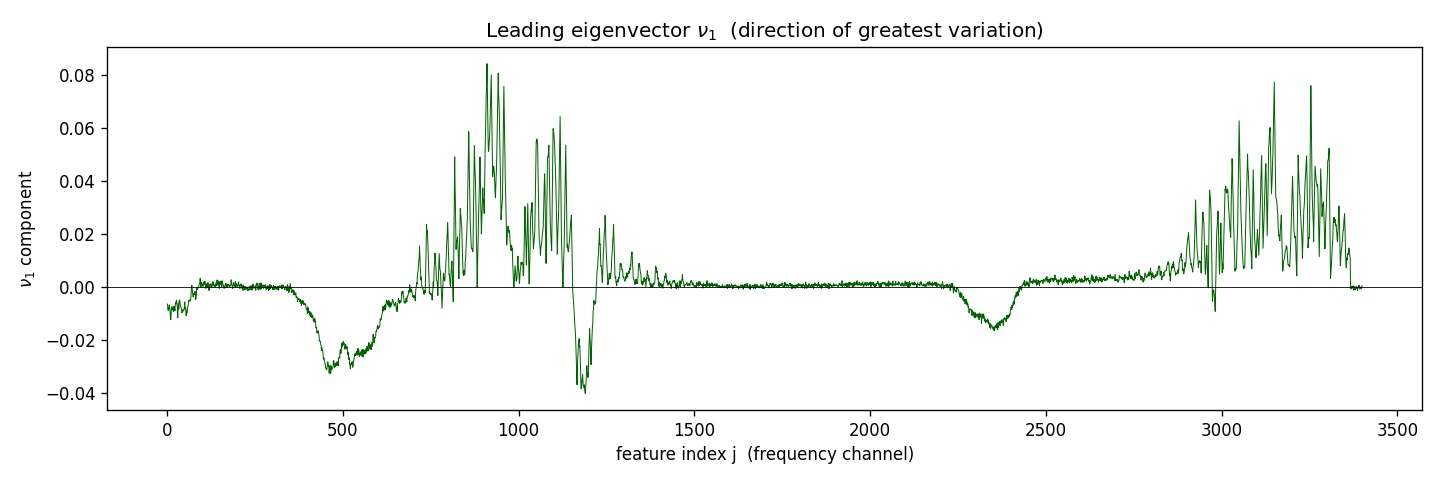
\includegraphics[width=0.84\linewidth]{q3d_v1.png}\\[3pt]

\includegraphics[width=0.84\linewidth]{q3d_v1_vs_row.png}
\caption{\emph{Top:} loadings of $\nu_1$, concentrated on two molecular bands with mixed signs
(a contrast direction). \emph{Bottom:} $\nu_1$ overlaid on the best-matching centred spectrum
($\cos\approx0.92$).}\label{fig:lead}
\end{figure}

% ======================================================================
\section{Part (e): clustering in covariance (feature) space}\label{sec:3e}
We now compress each vial to a handful of coordinates and look for groups. With
$V_4=[\nu_1\,\nu_2\,\nu_3\,\nu_4]$ (the top four eigenvectors of $C$), the compressed
coordinates are $Z=\Xt V_4\in\R^{\Nt\times4}$: row $z_i$ holds the four scores of vial $i$.
This is \textbf{dimensionality reduction} from $3401$ numbers to $4$, retaining the dominant
variation. We choose four because they lie within the eight signal directions of \S\ref{sec:3c}
yet are few enough to inspect as the $\binom42=6$ pairwise scatter plots
(Figure~\ref{fig:covscatter}), drawn with small, semi-transparent points so dense groups stay
visible.

The panels show many tight, well-separated blobs. Counting them by leader clustering (radius a
few multiples of the median nearest-neighbour spacing) gives $25$ clusters, and the count is
stable for radii from $6$ to $12$ times that spacing --- so it is a property of the data, not
of the threshold. Each blob is a set of vials with nearly identical spectra, i.e.\ one
concoction.

\begin{figure}[h]\centering

\includegraphics[width=0.92\linewidth]{q3e_covariance_scatter.png}
\caption{The six pairwise scatter plots of the top-4 covariance-space scores; each point is one
vial. The data resolves into $\approx25$ well-separated clusters.}\label{fig:covscatter}
\end{figure}

% ======================================================================
\section{Part (f): clustering in Gram (sample) space}\label{sec:3f}
The \textbf{Gram matrix} $G=\tfrac1{\Nt}\Xt\Xt\T$ is the $\Nt\times\Nt$ companion of $C$; its
entry $G_{ij}$ is the similarity between vials $i$ and $j$. Diagonalising $G$ confirms it shares
the nonzero eigenvalues of $C$ exactly (the top eight match to all printed digits), as Question
2d predicts. Its eigenvectors are already $\Nt$-dimensional, so \emph{each component is directly
a vial's coordinate} --- no projection of $\Xt$ is required. Scaling the eigenvectors by
$\sqrt{\Nt\lambda}=\sigma$ puts them in the same units as the covariance-space scores of
\S\ref{sec:3e}.

The same six scatter plots (Figure~\ref{fig:gramscatter}) and the same leader-clustering rule
again give $25$ clusters, stable over the same range of radii. The two scatter pictures
reproduce one another up to per-axis sign flips, because eigenvectors are defined only up to a
sign. We make this precise in the next section.

\begin{figure}[h]\centering

\includegraphics[width=0.92\linewidth]{q3f_gram_scatter.png}
\caption{The six pairwise scatter plots of the top-4 Gram-space coordinates. They reproduce the
covariance-space scatter of Figure~\ref{fig:covscatter} up to reflections, and again show
$\approx25$ clusters.}\label{fig:gramscatter}
\end{figure}

% ======================================================================
\section{Part (g): comparing the two approaches}\label{sec:3g}
\subsection{Do the two methods give the same number of clusters? Yes --- necessarily.}
Both routes return $25$ clusters, and this is forced by the algebra. The mathematical link: if
$C\nu=\lambda\nu$ then $\Xt\nu$ is an eigenvector of $G$ with the same eigenvalue $\lambda$, so
$C$ and $G$ share their nonzero eigenvalues. More strongly, with the SVD $\Xt=U\Sigma V\T$ the
covariance-space scores are $Z=\Xt V=U\Sigma$, while the (scaled) Gram coordinates are
$Z_g=U\sqrt{\Nt\lambda}=U\Sigma$. \textbf{Both coordinate sets are the same matrix $U\Sigma$},
identical up to the arbitrary sign of each eigenvector.

We verify this directly by correlating the two coordinate sets component by component
(Figure~\ref{fig:compare}): every matching component is perfectly correlated
($|\mathrm{corr}|=1.000$), all cross-correlations are $0$, and $|Z|=|Z_g|$ to machine
precision. Because the two point clouds are identical up to reflecting individual axes, the
clusters --- and hence their number --- must coincide. (In general the two pictures can differ
slightly when one matrix is numerically better conditioned, but here the structure is clean
enough that they agree exactly.)

\begin{figure}[h]\centering

\includegraphics[width=0.86\linewidth]{q3g_compare.png}
\caption{Comparison of the covariance-space (3e) and Gram-space (3f) coordinates: matching
principal components are perfectly correlated ($|\mathrm{corr}|=1$) and distinct ones are
uncorrelated, so the two scatter pictures are the same up to per-axis sign.}\label{fig:compare}
\end{figure}

\subsection{What does cluster membership \emph{mean} in each space?}
\textbf{Covariance space (3e).} A vial's coordinates are the projections of its centred
spectrum onto the top feature-space eigenvectors. Each coordinate says how strongly the vial
expresses one dominant \emph{pattern of spectral variation} (a weighted combination of
frequencies). Two vials are close when they express these patterns to the same degree, i.e.\
their spectra are similar mixtures along the directions where samples differ most. Covariance
space answers ``\emph{which mixture of frequencies does this vial express?}''

\textbf{Gram space (3f).} A vial's coordinates are the components of the top sample-space
eigenvectors of $G$. Since $G_{ij}$ is the similarity between vials $i$ and $j$, each Gram
eigenvector is a pattern over the $924$ vials, and a vial's coordinate is its loading in that
pattern --- a compressed summary of how similar it is to every other vial. Gram space answers
``\emph{which other vials does this one resemble?}''

Both place vials with near-identical spectra at the same point, so proximity in either
coordinate system means the underlying vials hold the same chemical concoction --- which is why
the two routes agree.

% ======================================================================
\section{Part (h): how many unique food samples are there?}\label{sec:3h}
Finally we count the genuine concoctions. We use all $960$ genuine vials --- the $40$ empty
blanks removed, but the $36$ high-norm vials \emph{kept}, because part (h) tells us the samples
are real fermented drinks, so that coherent, strongly-absorbing group is a genuine concentrated
concoction, not an error. (This is exactly why the removal in \S\ref{sec:3a} was kept
reversible.) We cluster in the top-$8$ signal subspace (the elbow of \S\ref{sec:3c}), which
denoises the data so that the groups separate cleanly.

Single-linkage connected components give \textbf{$26$ clusters}, and the count is completely
stable: it is $26$ for every threshold $\varepsilon$ from $0.25$ to $0.40$, and the leader
clustering of \S\ref{sec:3e}--\ref{sec:3f} agrees. The decisive evidence is the
\emph{replicate structure} (Figure~\ref{fig:sizes}): the clusters have sizes
$24\times37+2\times36=960$ --- about $37$ repeat measurements of each of $26$ distinct samples.
That clean, near-constant group size is the fingerprint of a designed experiment with $26$
unique concoctions, comfortably below the ``fewer than $100$'' stated in the prompt.

\begin{remark}
The covariance/Gram clusterings of \S\ref{sec:3e}--\ref{sec:3f} reported $25$ because they were
run on the $924$-vial set that \emph{excluded} the high-norm group. Restoring that one genuine
concoction gives $26$. This is the practical pay-off of having kept the cleaning decision
reversible.
\end{remark}

\begin{figure}[h]\centering
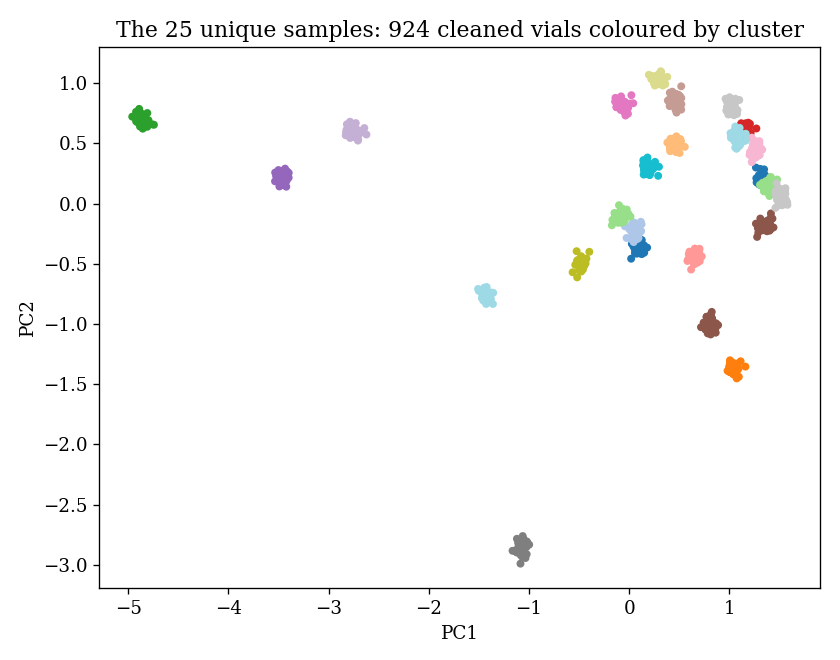
\includegraphics[width=0.92\linewidth]{q3h_clusters.png}
\caption{Cluster sizes for the $960$ genuine vials in the top-8 subspace: $26$ clusters of about
$37$ replicates each ($24\times37+2\times36=960$). The flat profile is the signature of a
designed $26$-sample experiment.}\label{fig:sizes}
\end{figure}

\subsection{Which earlier parts were useful?}
\begin{itemize}
\item \textbf{Part (a), cleaning.} Removing the $40$ empties was essential: left in, they would
form a spurious extra ``cluster'' of pure noise. Recognising the $36$ high-norm vials as a
\emph{real} sample (and keeping the removal reversible) is what turns $25$ into the correct
$26$.
\item \textbf{Part (c), the elbow.} $k^\star=8$ tells us the signal lives in $\sim8$ dimensions,
so we cluster in the top-$8$ principal components rather than the noisy $3401$. This denoising
is what makes the $26$ groups cleanly separable; clustering the raw spectra would be swamped by
noise. ($k^\star\approx8$ also echoes the $\sim10$ dominant molecules.)
\item \textbf{Parts (e), (f), (g).} These supply the cluster count, and the fact that the
covariance and Gram routes agree (g) shows the count is a real property of the data, not an
artefact of one method.
\item \textbf{Parts (b), (d).} These established that the data is low-dimensional and that the
leading directions are chemically meaningful contrasts, which justifies the
project-then-cluster pipeline.
\end{itemize}

% ======================================================================
\section{Conclusion}\label{sec:conclusion}
Starting from a raw $1000\times3401$ table, a short chain of linear-algebra tools recovered the
hidden structure of the experiment. We removed $40$ blank vials and $36$ anomalous ones
($\Nt=924$); found a total variance of $\tr(C)\approx7.90$ concentrated in a few molecular
bands; established by PCA that the data is strongly low-dimensional
($\lambda_1/\lambda_2\approx3.53$, an eight-dimensional signal subspace); interpreted the
leading direction as a chemical contrast; and, by clustering the genuine vials two
mathematically equivalent ways, determined that they comprise \textbf{$26$ unique food
samples}, each measured about $37$ times.

The same principle threads through all three questions of the challenge: a high-dimensional
system is governed by a small number of special directions. In Question 1 the dominant
eigenvector was a Markov chain's long-time steady state; in Question 2 the Power Method found
that direction by iteration, at a speed set by the spectral gap; and here in Question 3 the few
leading eigenvectors of the covariance (equivalently the Gram) matrix compressed $3401$-dimensional
spectra into a picture clear enough to count the drinks.

\appendix
% ======================================================================
\section{Glossary}\label{app:glossary}
\begin{description}[leftmargin=0pt,style=nextline]
\item[Sample / feature] a sample is one vial (a row of $X$); a feature is one frequency (a column).
\item[Norm $\norm{x}$] the length $\sqrt{\sum_j x_j^2}$ of a vector; a one-number measure of size.
\item[Transpose $X\T$] the matrix with rows and columns swapped.
\item[Mean-centering] subtracting each feature's average so every column averages zero.
\item[Variance] mean squared deviation from the mean; how much a feature varies across samples.
\item[Covariance matrix $C$] $\tfrac1{\Nt}\Xt\T\Xt$ ($M\times M$, feature space); diagonal = variances.
\item[Gram matrix $G$] $\tfrac1{\Nt}\Xt\Xt\T$ ($\Nt\times\Nt$, sample space); $G_{ij}$ = similarity of vials $i,j$.
\item[Trace] sum of the diagonal; for $C$ it is the total variance $=\sum\lambda_i$.
\item[Eigenvector / eigenvalue] a direction $v$ with $Cv=\lambda v$; $\lambda$ = variance along $v$.
\item[Spectral theorem] a real symmetric matrix has real eigenvalues and orthonormal eigenvectors.
\item[Positive semi-definite (PSD)] $w\T C w\ge0$ for all $w$; forces all $\lambda_i\ge0$.
\item[PCA] eigendecomposition of $C$; finds the directions of greatest variance.
\item[SVD] the factorisation $\Xt=U\Sigma V\T$; links $C$ ($V$) and $G$ ($U$) via $\sigma_i$.
\item[Scree plot / elbow] sorted eigenvalues; the elbow $k^\star$ separates signal from the noise floor.
\item[Spectral gap] $\lambda_1-\lambda_2$ (or $\lambda_1/\lambda_2$); a wide gap = one dominant direction.
\item[Score / projection] $z_i=\xt_i\cdot\nu$, a sample's coordinate along an eigenvector.
\item[Cosine similarity] $(a\cdot b)/(\norm a\norm b)$; scale-invariant comparison of direction.
\item[Cluster] a tight, well-separated group of points; here, vials of one concoction.
\end{description}

\section{Summary of key numerical results}\label{app:numbers}
\begin{center}\small
\begin{tabular}{ll}
\toprule
Quantity & Value \\
\midrule
File shape (as stored) & $(3401,1000)$; transposed, $M=3401$ (text says $3041$) \\
Empty vials removed (3a-i) & $40$ (rows $960$--$999$) \\
High-norm vials removed (3a-ii) & $36$ (rows $924$--$959$) \\
Cleaned samples $\Nt$ & $924$ \\
Exact-zero fraction (empty / real) & $50.2\%$ / $24.5\%$ \\
Max-variance feature $j^\star$ (3b) & $910$ (variance $\approx0.0199$) \\
Total variance $\tr(C)$ (3b) & $\approx7.90$ \\
Dominance ratio $\lambda_1/\lambda_2$ (3c) & $\approx3.53$ \\
Elbow $k^\star$ (3c) & $8$ (largest drop $\lambda_8/\lambda_9\approx4.1$) \\
Components for $95\%$ variance (3c) & $667$ \\
$\nu_1$ vs centred / raw / mean spectrum (3d) & $\cos\approx0.92$ / $0.67$ / $0.03$ \\
Clusters in covariance / Gram space (3e/3f) & $25$ / $25$ (on the $924$ set) \\
Cross-method correlation (3g) & $|\mathrm{corr}|=1$ matched, $0$ otherwise \\
\textbf{Unique food samples (3h)} & $\mathbf{26}$ ($\approx37$ replicates each) \\
\bottomrule
\end{tabular}
\end{center}

\end{document}
